\section{Ambiente di Lavoro}
\label{ambiente}
In questa sezione verrà illustrato in dettaglio l'ambiente di lavoro che il team \authorName{} utilizzerà durante lo sviluppo del progetto \project.

\subsection{Sistema operativo}
\label{sistema}
Il sistema operativo utilizzato per lo sviluppo del progetto è a discrezione di ogni singolo componente del gruppo. Questa scelta è dovuta principalmente al fatto che il progetto dovrà supportare più piattaforme.
\\In particolare i vari membri del gruppo utilizzeranno i seguenti sistemi operativi:
\begin{itemize}
\item Ubuntu 12.04 64bit;
\item Mac OS\glossario{} 10.9 64bit;
\item Windows\glossario{} 8 64bit.
\end{itemize}

\subsection{Coordinamento}
\label{coordinamento}
Il coordinamento del gruppo avviene tramite:
\begin{itemize}
\item Repository\glossario{} Git\glossario{};
\item Dropbox\glossario{};
\item Google Drive\glossario{};
\item Google Calendar\glossario{};
\item Jenkins.
\end{itemize}

\subsubsection{Repository Git}
\label{git}
Sono stati presi in considerazione vari repository\glossario{} (Git\glossario{}, Mercurial, SVN) prima di scegliere di utilizzare Git\glossario{}.
\\La scelta è ricaduta su Git\glossario{} per i seguenti motivi:
\begin{itemize}
\item La possibilità di poter lavorare localmente, senza bisogno di essere connessi a internet;
\item Git\glossario{} era già stato usato da vari membri del team;
\item La possibilità di ignorare certe estensioni dei file (gitignore);
\item La presenza di innumerevoli client, per chi non volesse utilizzarlo da shell.
\end{itemize}
Per i membri del gruppo, che non vogliono utilizzare la shell, sono consigliati i seguenti client:
\begin{itemize}
\item \textbf{Sourcetree:} disponibile per i sistemi Windows\glossario{} e Mac OS\glossario{};
\item \textbf{Giteye:} disponibile per  i sistemi Linux\glossario{}.
\end{itemize}

\subsubsection{Dropbox}
\label{dropbox}
In questo servizio cloud verranno messi tutti i file che non sono soggetti ad un controllo di versione.
\\Principalmente verrà utilizzato dai membri del gruppo per scambiarsi libri di testo, guide, ecc\dots .
\\La presenza del client ufficiale disponibile per la maggior parte dei sistemi operativi ha fatto cadere la scelta su questo servizio cloud.

\subsubsection{Google Drive}
\label{drive}
In quest'altro servizio cloud invece andranno messi tutti i documenti che:
\begin{itemize}
\item Non necessitano di alcun controllo di versione;
\item Necessitano di una forte interattività tra i vari membri del gruppo;
\item Sono accessibili direttamente da browser.
\end{itemize}
Principalmente Google Drive\glossario{} viene utilizzato per lavorare su dei file condivisi su Google Docs\glossario{}.
\\Un vantaggio di questo servizio è quello che i vari membri possono lavorare contemporaneamente sugli stessi documenti, tramite l'utilizzo di un browser.

\subsubsection{Google Calendar}
\label{calendar}
Google Calendar\glossario{} viene utilizzato dai membri del gruppo per la gestione delle risorse umane.
\\È stato creato un calendario condiviso tra i vari membri del gruppo, in modo da notificare:
\begin{itemize}
\item In quali date un certo membro non è disponibile;
\item In quali date c'è una riunione o un evento rilevante ai fini del gruppo.
\end{itemize}
Grazie alla gestione delle notifiche di Google Calendar\glossario{}, è possibile far in modo che 24 ore prima di un evento rilevante venga inviata una email a tutti i membri del gruppo come promemoria.

\subsubsection{Jenkins}
\label{jenkins}
Per svolgere l'\emph{integrazione continua} durante lo svolgimento del progetto si è deciso di appoggiarsi al servizio Jenkins\footnote{\url{http://jenkins-ci.org}}.
\\Si è scelto di utilizzare tale software per il gran numero di plugin.

\subsection{Pianificazione delle attività}
\label{pianificazione}
Per pianificare la gestione di progetto e gestire le risorse umane si è scelto di utilizzare GanttProject\glossario{}.
\\La scelta è ricaduta su tale applicativo per i seguenti motivi:
\begin{itemize}
	\item Portabilità, essendo il software scritto in Java;
	\item Open source;
	\item Permette la generazione di diagrammi di Gantt\glossario{} e delle risorse;
	\item Consente di esportare i diagrammi in formato \verb!PNG! o \verb!HTML!.
\end{itemize}

\subsection{Tracciamento bug}
\label{tracciamento bug}
Per il tracciamento dei bug\glossario{} è stato scelto di utilizzare l'applicativo web Mantis\footnote{\url{http://www.mantisbt.org}}.
\\Tale software è disponibile all'indirizzo: \url{http://sevenmonkeys.altervista.org/mantisbt/index.php}.
\\Mantis è accessibile a tutti i membri del gruppo \authorName{} tramite login e password.
\begin{figure}
	\centering
	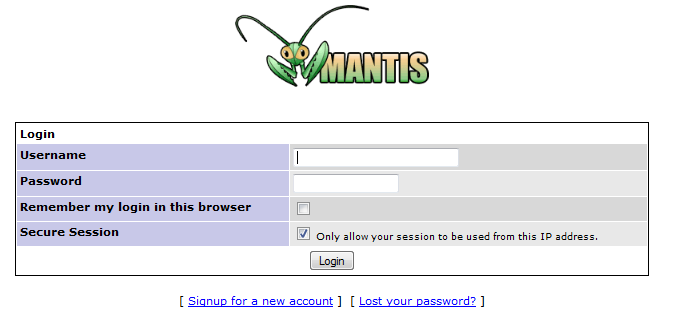
\includegraphics[width=10cm]{./content/Immagini/mantis.png}
	\caption{Schermata di login di mantis}
	\label{login_password}
\end{figure}

\subsection{ReqMonkeys}
\label{reqmonkeys}
Per facilitare il tracciamento dei requisiti è stato creata dal \administrator{} il software \textbf{ReqMonkeys}, il quale è ospitato nel sito del gruppo all'indirizzo \url{sevenmonkeys.altervista.org}.
\\Il software permette di gestire il tracciamento e gestire requisiti, casi d'uso, fonti, test d'unità velocizzando le varie operazioni.
\\Nella figura sottostante è possibile vedere l'interfaccia della pagina principale di \textbf{ReqMonkeys}. 
%\begin{figure}
%	\centering
%	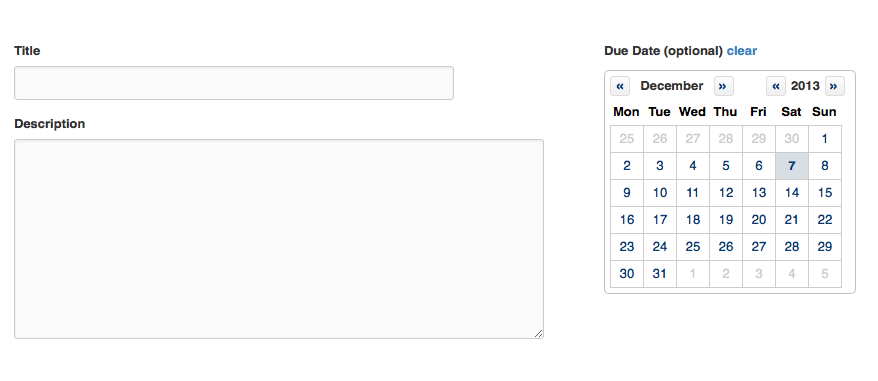
\includegraphics{{./content/Immagini/Screen1.png}
%	\caption{ReqMonkeys: pagina principale}
%	\label{ReqMonkeys}
%\end{figure}

\subsubsection{Analisi dei Requisiti}
\label{analisi_requisiti_trax}
\textbf{ReqMonkeys} permette di tracciare i requisiti.
\\Infine il software permette di scaricare il file \LaTeX{} \verb!Requisiti.tex! contenente le tabelle.

\subsection{Strumenti per i documenti}
\label{ambdoc}

\subsubsection{\LaTeX}
\label{stesura}
Per la scrittura dei documenti è stato scelto di utilizzare il linguaggio di markup\glossario{} \LaTeX \footnote{\url{http://latex-project.org/ftp.html}}.
\\Come editor è consigliato l'utilizzo di \TeX maker\footnote{\url{http://www.xm1math.net/texmaker/}}, il quale è disponibile per tutti i principali sistemi operativi.

\subsubsection{Script}
\label{script}
Per semplificare alcune azioni l'\administrator{}  ha creato alcuni script.
\\Per facilitare la compilazione e il controllo dei documenti è stato creato un Makefile, disponibile nel repository\glossario{} (\textit{/Scripts/Makefile}).
\\Il Makefile consente di:
\begin{itemize}
\item \textbf{Generazione di tutti i PDF:} tramite il comando \verb!make RP! verranno generati tutti i \verb!PDF!\glossario{} e salvati sulla cartella \verb!Consegne/RR!;
\item \textbf{Eseguire il controllo ortografico:} tramite il comando \verb!make aspell! verrà invocato l'applicativo Aspell\glossario{} su tutti i documenti;
\item \textbf{Eliminare i file generati:} tramite il comando \verb!make clean! verranno eliminati tutti i file generati da vecchie compilazioni.
\end{itemize}

\subsubsection{Controllo ortografico}
\label{verortografica}
Per la verifica ortografica dei documenti scritti in \LaTeX{} verrà utilizzato l'applicativo Aspell\glossario{}. La scelta è ricaduta su di esso, piuttosto che sul correttore ortografico integrato in \TeX{}maker, perché consente di aggiungere termini al proprio dizionario.
\\L'uso di Aspell\glossario{} avverrà direttamente da shell tramite l'uso del comando:
\begin{verbatim}
aspell --mode=tex --lang=it check nomedocumento.tex
\end{verbatim}

\subsubsection{Diagrammi UML}
\label{UML}
Per quanto riguarda la modellazione dei diagrammi dei casi d'uso, diagrammi di attività e diagrammi di sequenza, si è deciso di adottare il software \textit{Astah}\glossario{} - \textit{Professional Edition}. Quest'ultimo è uno strumento multipiattaforma che permette di disegnare svariate tipologie di grafici secondo lo standard UML2.0\glossario{}.\\
Per la realizzazione dei diagrammi delle classi e dei package\glossario{} verrà utilizzato il software Visual Paradigm\footnote{\url{http://www.visual-paradigm.com}}. Tale software offre i seguenti vantaggi:
\begin{itemize}
	\item Distinzione tra i diagrammi delle classi e package\glossario{};
	\item Il software è multipiattaforma;
	\item Generazione automatica del codice dello \lq\lq{}scheletro\rq\rq{} delle classi;
	\item Facilità di utilizzo del software.
\end{itemize}

\subsection{Strumenti per lo sviluppo}
\label{ambientesviluppo}
L'\administrator{} ha configurato una macchina virtuale Windows\glossario{} utilizzando il software \textbf{VirtualBox}\footnote{\url{https://www.virtualbox.org}}.
\\La macchina virtuale contiene tutto il software di lavoro utilizzato dal gruppo \authorName{}.
\\Come sistema operativo è stato scelto Windows\glossario{} in quanto lo sviluppo principale di \project{} deve avvenire per tale sistema.

\subsubsection{Framework}
\label{framework}
Per la realizzazione della grafica del progetto è stato scelto di utilizzare il framework\glossario{} Qt\glossario{}.
I motivi che hanno portato a tale scelta sono:
\begin{itemize}
\item \textbf{Qt Linguistic:} è disponibile un tool\glossario{}, che permette il supporto a varie lingue;
\item \textbf{Qt Designer:} è presente questo tool\glossario{}, il quale facilita la creazione di interfacce;
\item \textbf{Esperienza:} tutti i membri del team hanno già utilizzato il framework\glossario{} Qt\glossario{} in precedenza nel corso di Programmazione ad Oggetti.
\end{itemize}
La versione utilizzata delle librerie Qt\glossario{} è la 5.1.

\subsubsection{Librerie}
\label{librerie}
Per la realizzazione di alcune parti fondamentali del progetto, verranno utilizzate delle librerie esterne al framework\glossario{} sopra descritto, come suggerito dai proponenti. In particolare verranno impiegate le librerie ITK\glossario{} (v4.5.0) e VTK\glossario{} (v6.1.0) per la manipolazione dei vari formati d'immagine che il software dovrà saper gestire. Queste librerie offrono la possibilità di importare ed esportare le immagini all'interno del software, e di poter quindi applicarne gli algoritmi che effettuano i calcoli voluti. 

\subsubsection{Ambiente di codifica}
\label{ambientecodifica}
Per la scrittura del codice è stato scelto di utilizzare l'IDE\glossario{} Qt\glossario{} Creator.
\\È stato scelto poiché, oltre ad integrarsi direttamente con le librerie Qt\glossario{}, fornisce degli strumenti di editing, debugging e la possibilità di utilizzare la documentazione ufficiale anche offline.
\\Inoltre Qt\glossario{} Creator si integra con Git\glossario{}.
\\La versione di Qt\glossario{} Creator utilizzata è la 2.8.1.

\subsubsection{Documentazione}
\label{documentazione_codice}
Per la documentazione del codice è stato scelto di usare il sistema Doxygen\footnote{\url{http://www.stack.nl/~dimitri/doxygen/}}, il quale permette una generazione automatica della documentazione a partire dal codice.
\\Il sistema estrae la documentazione dai commenti inseriti nel codice sorgente e dalla dichiarazione delle strutture dati.
\\Doxygen permette di generare la documentazione in formato \verb!HTML! o \LaTeX.